\documentclass{beamer}
\usepackage[T2A]{fontenc}
\usepackage[utf8]{inputenc}
\usepackage{cmap}
\usepackage[english,russian]{babel}
\usepackage{amssymb, latexsym, amsmath, textcomp}
\usepackage{listings}
\usepackage{multicol}
%\usepackage{graphicx}
%\setbeamercovered{dynamic}
\usefonttheme{serif}
\usepackage{indentfirst}
%\lstset{extendedchars=\true}

\begin{document}


\title{Знакомство с \LaTeX}
\author{Платонова Е. В.}
\institute{Московский авиационный институт}
\date{2012}
\frame{\titlepage}

\begin{frame}
  \frametitle{Что такое \LaTeX ?}
\begin{itemize}
\item \TeX\ --- это созданная американским математиком и программистом Дональдом Кнутом система для верстки технических текстов.

\item \LaTeX\ --- издательская система на базе \TeX 'а.
\end{itemize}
\end{frame}


\begin{frame}
  \frametitle{Почему \LaTeX ?}
\begin{itemize}
\item Напечатанный текст выглядит «совсем как в книге»: достигается лучшее качество полиграфии.
\item Переносимый: исходник — обычный текст.
\item Легкий набор формул.
\item Свободный и бесплатный.
\item Кроссплатформенный: работает как под Windows, так и под Unix.
\item Расширяемый: множество подключаемых модулей.
\item Является стандартом во многих научных сферах.
\end{itemize}
\end{frame}

\begin{frame}
  \frametitle{\LaTeX\ работает не в WISIWIG-режиме}
  
  WISIWIG — «What you see is what you get».
  \\
  Невизуальный режим напоминает «программирование документа».

\end{frame}

\begin{frame}
  \frametitle{Ближе к делу: простой пример}
  \begin{columns}
    \begin{column}{0.5\textwidth}
      \begin{figure}[h!]
        \centering{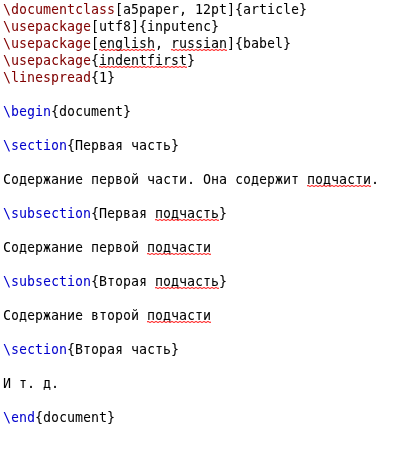
\includegraphics[scale=0.4]{pics/easy-tex.png}}
      \end{figure}
    \end{column}
    \begin{column}{0.5\textwidth}
      \begin{figure}[h!]
        \centering{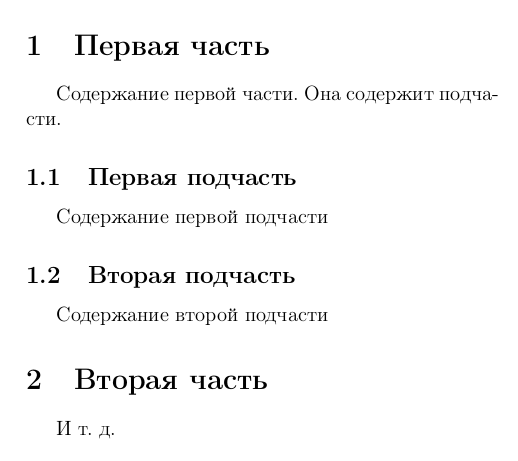
\includegraphics[scale=0.3]{pics/easy-pdf.png}}
      \end{figure}
    \end{column}
  \end{columns}
\end{frame}


\begin{frame}
  \frametitle{Списки}
  \begin{columns}
    \begin{column}{0.5\textwidth}
      \begin{figure}[h!]
        \centering{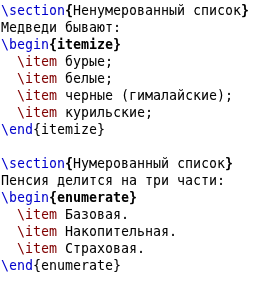
\includegraphics[scale=0.4]{pics/lists-tex.png}}
      \end{figure}
    \end{column}
    \begin{column}{0.5\textwidth}
      \begin{figure}[h!]
        \centering{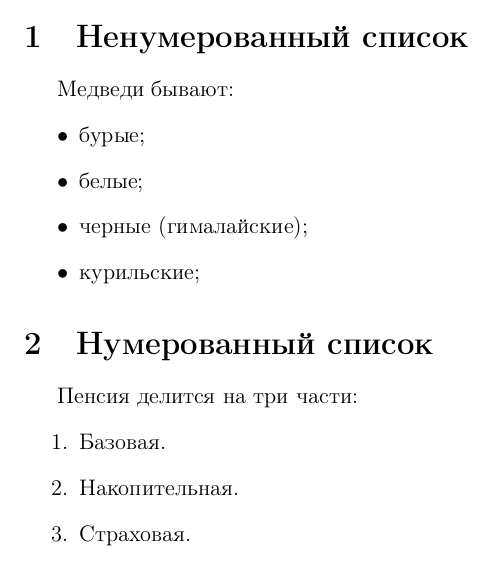
\includegraphics[scale=0.3]{pics/lists-pdf.png}}
      \end{figure}
    \end{column}
  \end{columns}  
\end{frame}


\begin{frame}
  \frametitle{Набор формул}
  \begin{columns}
    \begin{column}{0.5\textwidth}
      \begin{figure}[h!]
        \centering{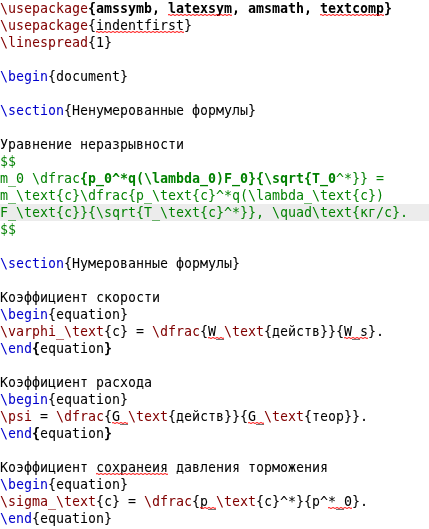
\includegraphics[scale=0.37]{pics/formulas-tex.png}}
      \end{figure}
    \end{column}
    \begin{column}{0.5\textwidth}
      \begin{figure}[h!]
        \centering{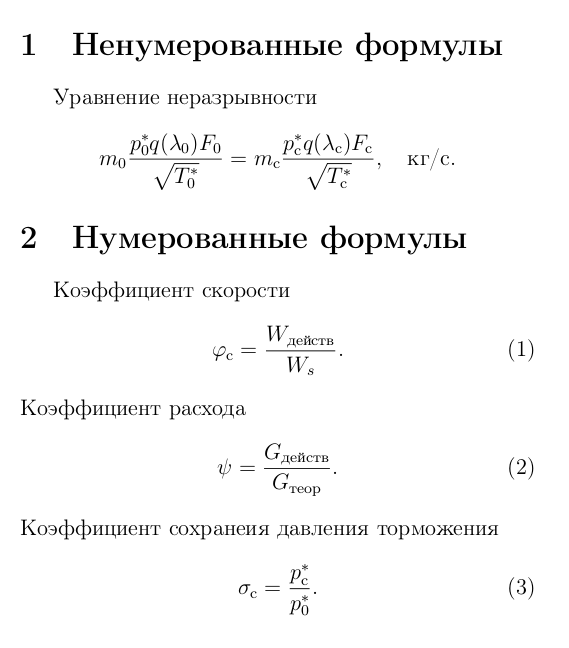
\includegraphics[scale=0.3]{pics/formulas-pdf.png}}
      \end{figure}
    \end{column}
  \end{columns}  
\end{frame}


\begin{frame}
  \frametitle{Как вставлять рисунки?}
  \begin{columns}
    \begin{column}{0.5\textwidth}
      \begin{figure}[h!]
        \centering{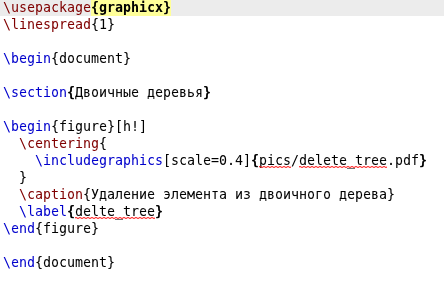
\includegraphics[scale=0.37]{pics/figures-tex.png}}
      \end{figure}
    \end{column}
    \begin{column}{0.5\textwidth}
\section{Двоичные деревья}

\begin{figure}[h!]
  \centering{
    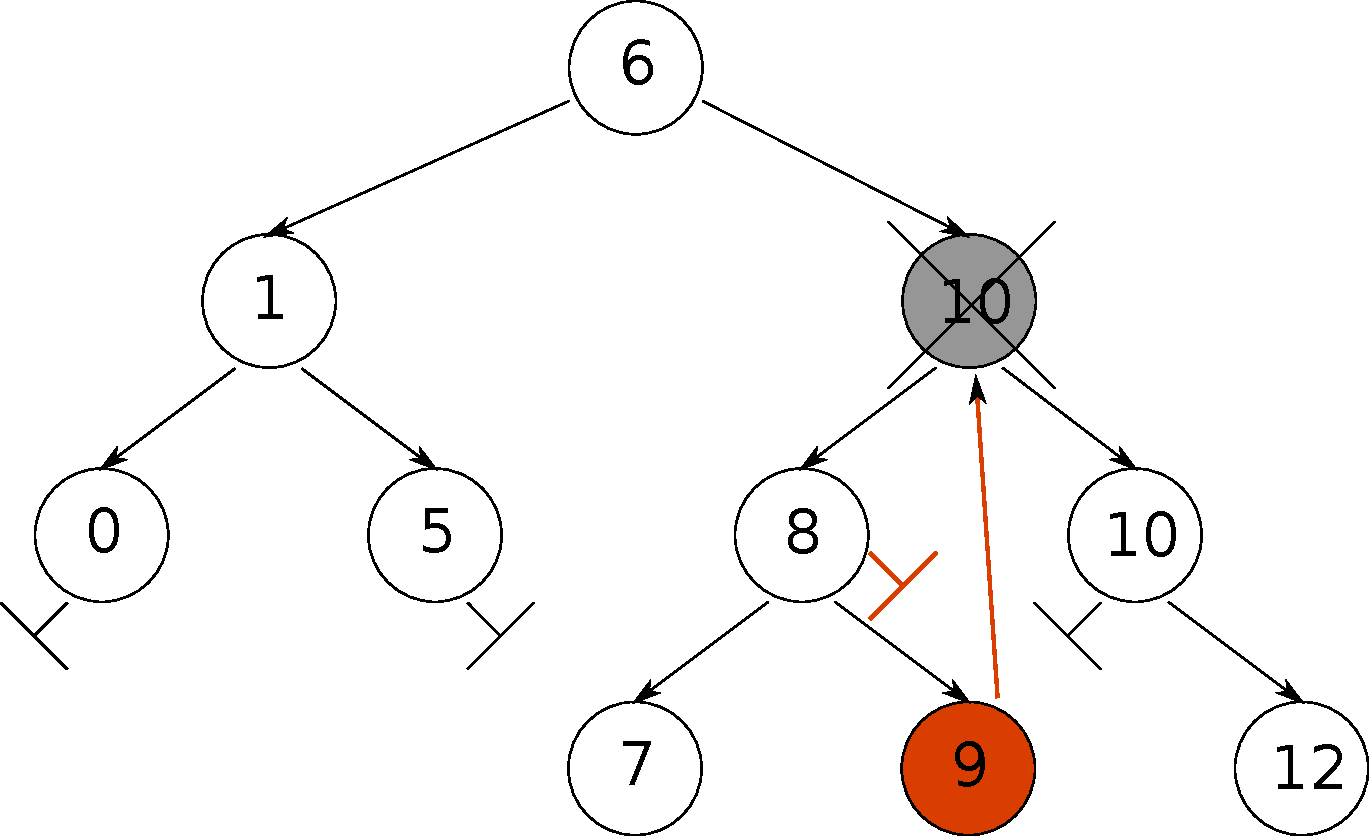
\includegraphics[scale=0.2]{pics/delete_tree.pdf}
  }
  \caption{Удаление элемента из двоичного дерева}
  \label{delte_tree}
\end{figure}
    \end{column}
  \end{columns}  
\end{frame}

\begin{frame}
  \frametitle{Таблицы}
  \begin{columns}
    \begin{column}{0.5\textwidth}
      \begin{figure}[h!]
        \centering{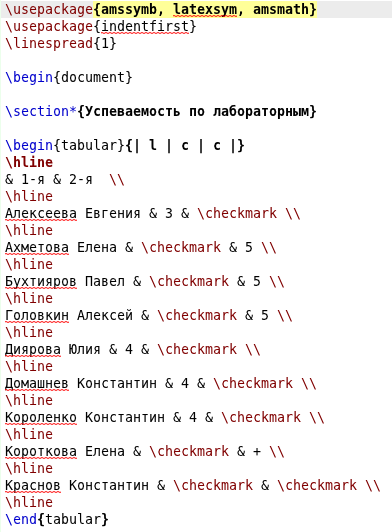
\includegraphics[scale=0.37]{pics/tabulars-tex.png}}
      \end{figure}
    \end{column}
    \begin{column}{0.5\textwidth}
      \begin{figure}[h!]
        \centering{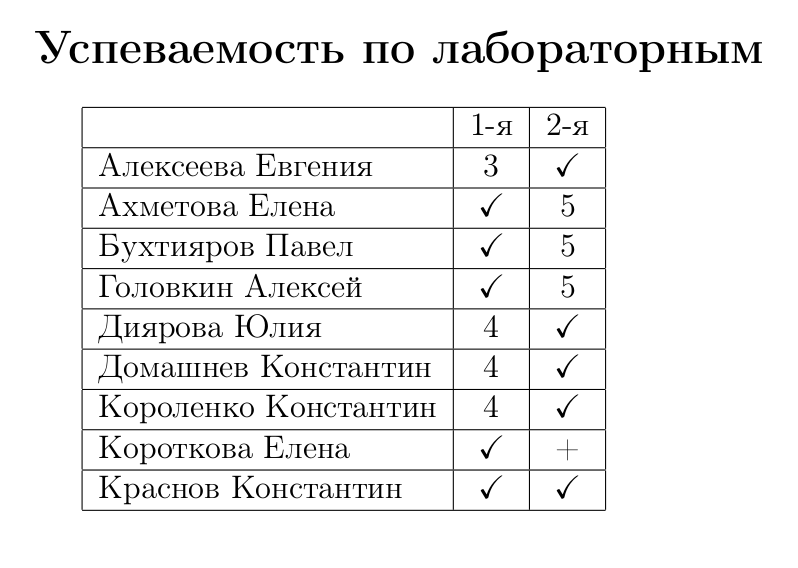
\includegraphics[scale=0.2]{pics/tabulars-pdf.png}}
      \end{figure}
    \end{column}
  \end{columns}  
\end{frame}

\begin{frame}
  \frametitle{Классы документов}
  \begin{itemize}
    \item Для научной статьи — article.
    \item Для книги — book;
    \item Для презентации — beamer.
  \end{itemize} 
\end{frame}

\begin{frame}
  \frametitle{Beamer}
  Эта презентация сделана с помощью \LaTeX 'а!
  \begin{figure}[h!]
    \centering{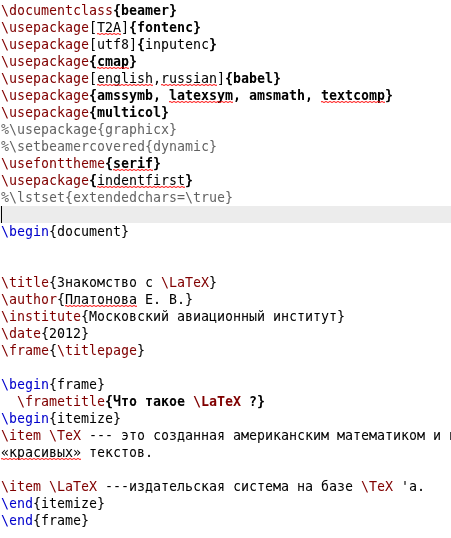
\includegraphics[scale=0.37]{pics/beamer-tex.png}}
  \end{figure}
\end{frame}

\begin{frame}
  \frametitle{Дистрибутивы \LaTeX 'а}
  \begin{itemize}
    \item Для Unix — Texlive;
    \item Для Windows — Miktex.
  \end{itemize} 
\end{frame}

\begin{frame}
  \frametitle{Редакторы для \LaTeX 'а}
  \begin{itemize}
    \item Emacs, Gedit, Notepad++ и пр.;
    \item Texmaker.
  \end{itemize} 
\end{frame}
  
\begin{frame}
  \frametitle{Texmaker — удобный редактор}
  \begin{figure}[h!]
    \centering{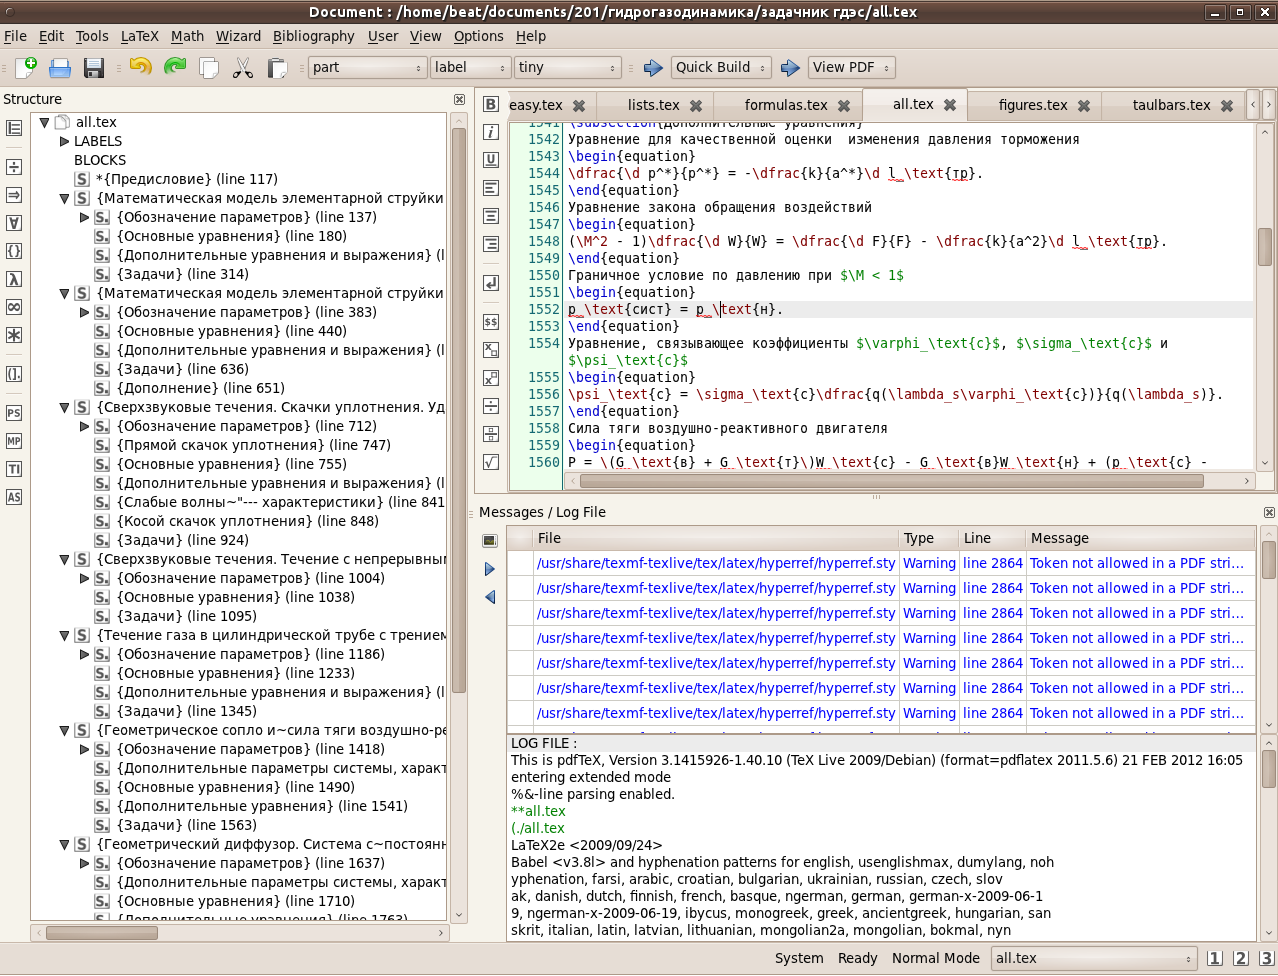
\includegraphics[scale=0.2]{pics/texmaker.png}}
  \end{figure}
\end{frame}

\begin{frame}
  \frametitle{Компиляция}
  \begin{itemize}
    \item \textbf{latex} name.tex $\rightarrow$ name.dvi; \textbf{dvips} name.dvi $\rightarrow$ name.ps; \textbf{ps2pdf} name.ps $\rightarrow$ name.pdf.
    \item \textbf{pdflatex} name.tex $\rightarrow$ name.pdf.
  \end{itemize}   
\end{frame}

\begin{frame}
  \frametitle{Особенности верстки}

  \begin{itemize}  
  \item Тире, минус и дефис~— разные символы (—, $-$, -):
    \begin{itemize}
    \item \LaTeX~— система для верстки технических текстов.
    \item $5 - 5 = 0$
    \item Питон поддерживает объектно-ориентированный стиль программирования.
    \end{itemize}
  \item Кавычки-елочки и кавычки-лапки:
    \begin{itemize}
    \item «Я не могу заказать блюдо в ресторане потому, что постоянно смотрю на шрифты в меню.» Д. Кнут.
    \item «На ночь я всегда читаю ''Искусство программирования``,» — сказал бы типичный студент.
    \item "\ " — вообще не кавычки.
    \end{itemize}
  \item Пробелы не ставятся перед знаками препинания и ставятся после. Исключение составляет тире: пробел ставится в обоих случаях.
  \end{itemize}
\end{frame}

\begin{frame}
  \frametitle{Скобки в формулах}

      $$
      \left(
       \left[
        \left\langle
         \left\{
           \left\lceil
            \left|
             \left\lfloor
              \text{text}^{10}
             \right\rfloor^9
            \right|^8
           \right\rceil^7
         \right\}^6
        \right\rangle^5
       \right]^4
      \right)^3
      $$
    
      {\it Неверно:}
      $$
      \frac{1}{\sigma \sqrt{2 \pi}} \exp( - \frac{( x - \mu ) ^ 2}{2 \sigma ^ 2} )
      $$
      {\it Верно:}
      $$
      \frac{1}{\sigma \sqrt{2 \pi}} \exp\left( - \frac{\left( x - \mu \right) ^ 2}{2 \sigma ^ 2} \right)
      $$
      
          \begin{center}{\small(Функция распределения Гаусса)}\end{center}

\end{frame}

\begin{frame}
  \frametitle{Пробелы}
  \begin{itemize}
  \item Тонкая шпация или малый пробел \textbackslash , \\
    Иванов И.И.~— {\it неверно} \\
    Иванов И. И.~— {\it неверно}\\
    Иванов И.\,И.~— {\it верно}
  \item Неразрывный пробел $\sim$\\
    Если слово нельзя перенести на другую строку: Иванов$\sim$И.
  \end{itemize}

\end{frame}

\begin{frame}
  \frametitle{Размеры букв}
  \begin{columns}
    \begin{column}{0.5\textwidth}
      \textbackslash tiny Малюсенький\\
      \textbackslash small Маленький\\
      \textbackslash normal Нормальный\\
      \textbackslash large Большой\\
      \textbackslash Large Побольше\\
      \textbackslash LARGE Очень большой\\
      \textbackslash huge Огромный\\
      \textbackslash Huge Гигантский\\
    \end{column}
    \begin{column}{0.5\textwidth}
      {\tiny Малюсенький} \\
      {\small Маленький} \\
      Нормальный \\
      {\large Большой} \\
      {\Large Побольше} \\
      {\LARGE Очень большой} \\
      {\huge Огромный} \\
      {\Huge Гигантский}
    \end{column}
  \end{columns}

\end{frame}

\begin{frame}
  \frametitle{Начертания букв}
  \begin{columns}
    \begin{column}{0.65\textwidth}
      \textbackslash textrm \{Прямое\} \\
      \textbackslash textsl \{Наклонное\} \\
      \textbackslash textit \{Курсивное\} \\
      \textbackslash textsf \{Рубленное(без засечек)\} \\
      \textbackslash textsc \{Капитель\} \\
      \textbackslash textbf \{Жирное\} \\
    \end{column}
    \begin{column}{0.45\textwidth}
      \textrm{Прямое} \\
      \textsl{Наклонное} \\
      \textit{Курсивное} \\
      \textsf{Рубленное (без засечек)} \\
      \textsc{Капитель} \\
      \textbf{Жирное} \\
    \end{column}
  \end{columns}

\end{frame}

\begin{frame}
  \frametitle{Если верстаете в \LaTeX 'е — делайте это красиво.}
  {\large Плохие советы:}
  \begin{itemize}
  \item Ставьте много восклицательных знаков!!!!!
  \item С вопросительными, думаете, нужно по-другому??????
  \item И пробелы,друзья мои,не нужны.
  \item Тире и дефис можно не различать!!! — и - одно и то же!!!
  \item "\ " — используйте эти «кавычки».
  \item Ч\texttt{\textit{ем}} {\tiny Б}{\large 0}{\tiny Л}ьш{\tiny Е} на\textit{чЕ}{\tiny р}тан\textbf{и}й  Вы \textsf{ис}\textsc{по}\textit{ль}{\LARGE з}у\textsl{е}те,тем л\textit{уч}ше {\tiny ч}ит\textbf{\textit{А}}ется в{\LARGE а}ш {\tiny те}{\large к}ст!!\textit{!}!\textbf{!}
  \end{itemize} 
  Типичный пример:\\
$$\boxed{  I = \dfrac{U}{R}\text{-\textbf{\textit{самая ВАЖНАЯ \large формула}!!!!}}}$$
\end{frame}

\begin{frame}
  \begin{center}
    Перейдем к демонстрации!
  \end{center}

\end{frame}

\end{document}